\subsection*{Problema 42}

\textbf{Enunciado:} \\
Calcular la integral indefinida:
\begin{align*}
I = \int x^{3/2} \left(2x^{1/3} - 1\right)^3 dx
\end{align*}

\textbf{Solución:} \\
Para resolver la integral, primero desarrollamos el binomio al cubo dentro del integrando. 
Recordemos la identidad del binomio:
\begin{align*}
(a - b)^3 = a^3 - 3a^2b + 3ab^2 - b^3
\end{align*}

Aplicando esta identidad con $a = 2x^{1/3}$ y $b = 1$, obtenemos:
\begin{align*}
\left(2x^{1/3} - 1\right)^3 &= (2x^{1/3})^3 - 3(2x^{1/3})^2(1) \\
&\quad + 3(2x^{1/3})(1)^2 - (1)^3
\end{align*}

Simplificando cada uno de los términos del desarrollo:
\begin{align*}
\left(2x^{1/3} - 1\right)^3 &= 8x - 12x^{2/3} + 6x^{1/3} - 1
\end{align*}

Sustituimos este resultado de vuelta en la integral original:
\begin{align*}
I &= \int x^{3/2} \Big(8x - 12x^{2/3} \\
&\quad + 6x^{1/3} - 1\Big) dx
\end{align*}

A continuación, distribuimos $x^{3/2}$ a cada término utilizando las leyes de los exponentes ($x^m \cdot x^n = x^{m+n}$):
\begin{align*}
8x^{3/2} \cdot x^1 &= 8x^{5/2} \\
-12x^{3/2} \cdot x^{2/3} &= -12x^{13/6} \\
6x^{3/2} \cdot x^{1/3} &= 6x^{11/6} \\
-1 \cdot x^{3/2} &= -x^{3/2}
\end{align*}

Reescribimos la integral con la suma de términos simplificados:
\begin{align*}
I &= \int \Big( 8x^{5/2} - 12x^{13/6} \\
&\quad + 6x^{11/6} - x^{3/2} \Big) dx
\end{align*}

Aplicamos la regla de la potencia para la integración $\int x^n dx = \frac{x^{n+1}}{n+1}$ término a término:

1. Para el primer término:
\begin{align*}
\int 8x^{5/2} dx &= 8 \left(\dfrac{x^{7/2}}{7/2}\right) = \dfrac{16}{7}x^{7/2}
\end{align*}

2. Para el segundo término:
\begin{align*}
\int -12x^{13/6} dx &= -12 \left(\dfrac{x^{19/6}}{19/6}\right) \\
&= -\dfrac{72}{19}x^{19/6}
\end{align*}

3. Para el tercer término:
\begin{align*}
\int 6x^{11/6} dx &= 6 \left(\dfrac{x^{17/6}}{17/6}\right) = \dfrac{36}{17}x^{17/6}
\end{align*}

4. Para el cuarto término:
\begin{align*}
\int -x^{3/2} dx &= -\dfrac{x^{5/2}}{5/2} = -\dfrac{2}{5}x^{5/2}
\end{align*}

Combinando todos los resultados y agregando la constante de integración $C$, obtenemos la solución general:
\begin{align*}
I &= \dfrac{16}{7}x^{7/2} - \dfrac{72}{19}x^{19/6} \\
&\quad + \dfrac{36}{17}x^{17/6} - \dfrac{2}{5}x^{5/2} + C
\end{align*}

\begin{figure}[H]
	\centering
	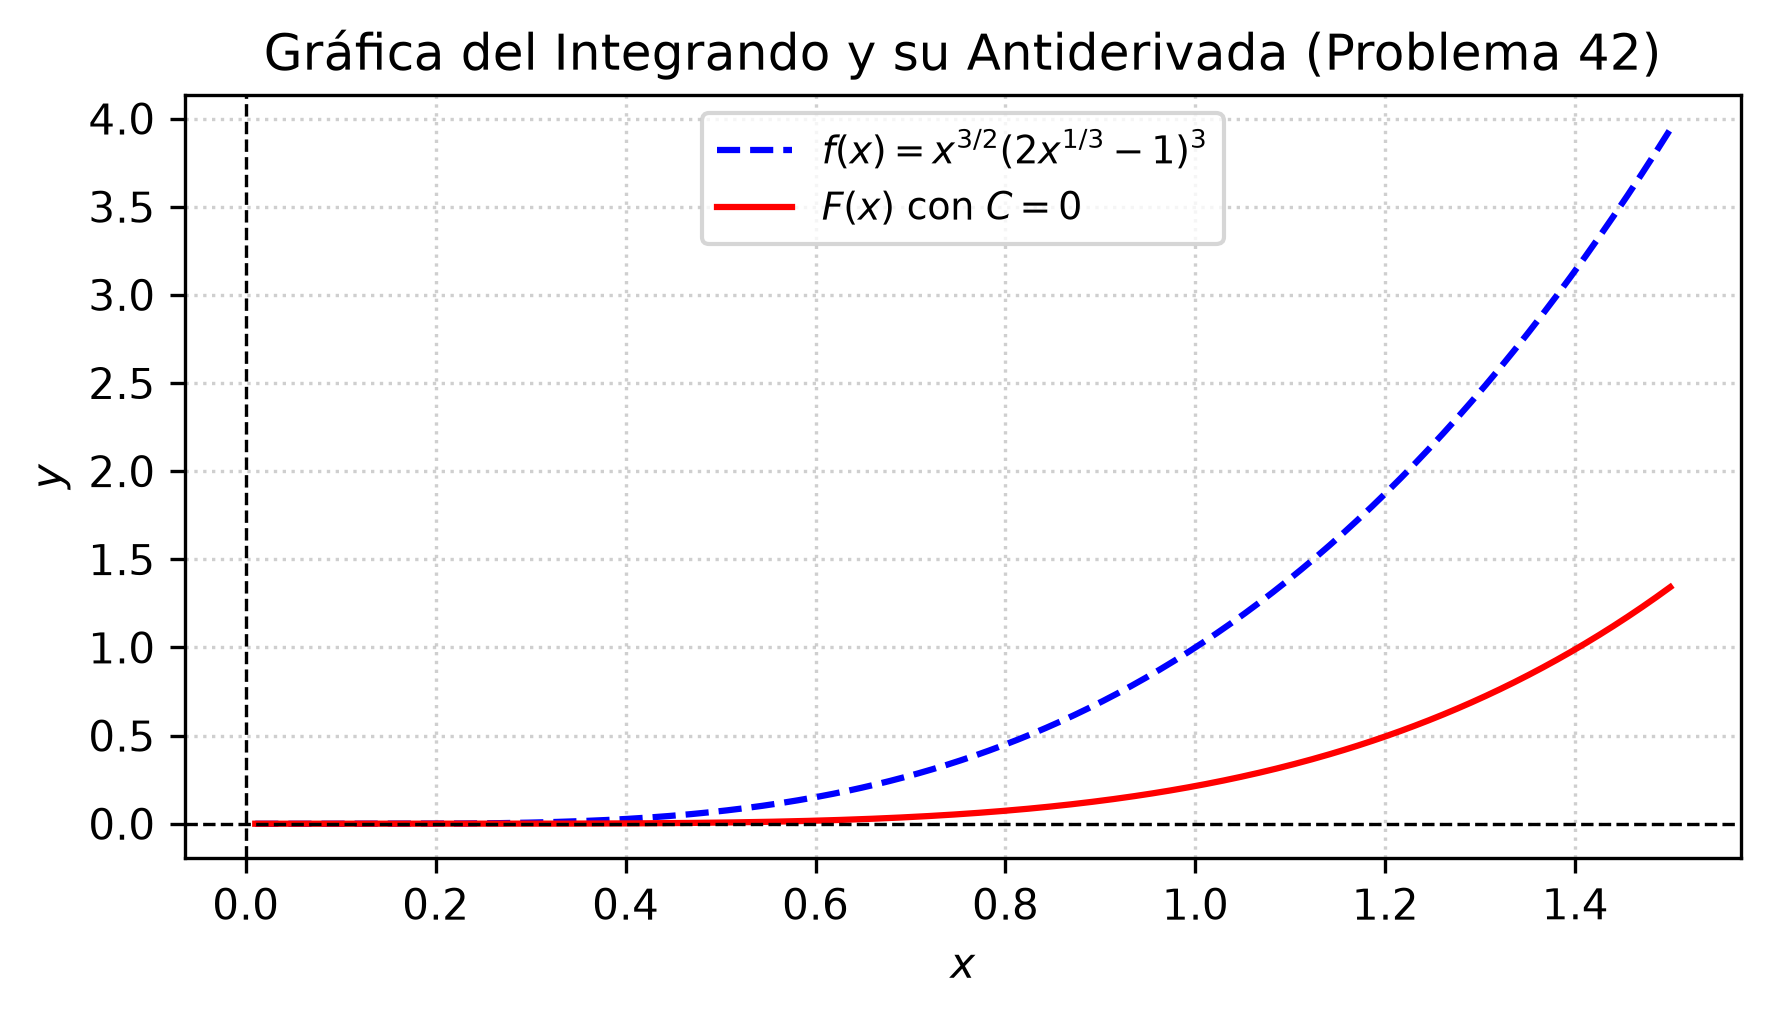
\includegraphics[width=\columnwidth]{semana_05/graficas/SEM05_P42_grafica.png}
	\caption{Representación gráfica de $f(x)$ y su antiderivada $F(x)$ evaluada para la constante de integración $C = 0$ (Problema 42).}
	\label{fig:problema42}
\end{figure}
